\documentclass[tikz]{standalone}
\begin{document}
\begin{tikzpicture}
    \node[anchor=south west,inner sep=0] at (0,0) {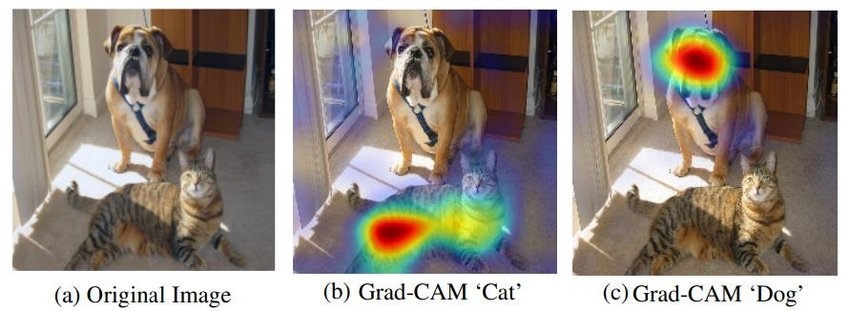
\includegraphics[width=\textwidth]{tikz/chapter5 - GradCam Image.png}};
    \node[rectangle, fill=white, draw=white, anchor=south west, minimum width=12cm, minimum height=0.6cm] at (0.1,-0.2) {};
    \node[fill=white, anchor=south west, align=center] at (0.77,-0.12) {Original Image};
    \node[fill=white, anchor=south west, align=center] at (4.5,-0.06) {Grad-CAM "Cat"};
    \node[fill=white, anchor=south west, align=center] at (8.55,-0.12) {Grad-CAM "Dog"};
\end{tikzpicture}
\end{document}